\documentclass[]{article}

% Imported Packages
%------------------------------------------------------------------------------
\usepackage{amssymb}
\usepackage{amstext}
\usepackage{amsthm}
\usepackage{amsmath}
\usepackage{enumerate}
\usepackage{fancyhdr}
\usepackage[margin=1in]{geometry}
\usepackage{graphicx}
\usepackage{float} % added to insert tables & figures in the place they are written
%\usepackage{extarrows}
%\usepackage{setspace}
%------------------------------------------------------------------------------

% Header and Footer
%------------------------------------------------------------------------------
\pagestyle{plain}  
\renewcommand\headrulewidth{0.4pt}                                      
\renewcommand\footrulewidth{0.4pt}                                    
%------------------------------------------------------------------------------

% Title Details
%------------------------------------------------------------------------------
\title{Deliverable \#2 Template}
\author{SE 3A04: Software Design III -- Large System Design}
\date{}                               
%------------------------------------------------------------------------------

% Document
%------------------------------------------------------------------------------
\begin{document}

\maketitle	
\noindent{\bf Tutorial Number:} T01\\
{\bf Group Number:} G01 \\
{\bf Group Members:} 
\begin{itemize}
	\item Benjamin Bloomfield
	\item Vikram Chandar
    \item Trisha Panchal
    \item Yug Vashisth
    \item Hamza Nadeem
\end{itemize}

\section*{IMPORTANT NOTES}
\begin{itemize}
	%	\item You do \underline{NOT} need to provide a text explanation of each diagram; the diagram should speak for itself
	\item Please document any non-standard notations that you may have used
	\begin{itemize}
		\item \emph{Rule of Thumb}: if you feel there is any doubt surrounding the meaning of your notations, document them
	\end{itemize}
	\item Some diagrams may be difficult to fit into one page
	\begin{itemize}
		\item Ensure that the text is readable when printed, or when viewed at 100\% on a regular laptop-sized screen.
		\item If you need to break a diagram onto multiple pages, please adopt a system of doing so and thoroughly explain how it can be reconnected from one page to the next; if you are unsure about this, please ask about it
	\end{itemize}
	\item Please submit the latest version of Deliverable 1 with Deliverable 2
	\begin{itemize}
		\item Indicate any changes you made.
	\end{itemize}
	\item If you do \underline{NOT} have a Division of Labour sheet, your deliverable will \underline{NOT} be marked
\end{itemize}

\newpage
\section{Introduction}
\label{sec:introduction}
% Begin Section

This section should provide an brief overview of the entire document.

\subsection{Purpose}
\label{sub:purpose}
% Begin SubSection
% State the purpose and intended audience for the document.\\\\
This document is intended to provide a high-level overview of the SCEMAS system architecture design as well as considerations for various subsystems that are a part of SCEMAS.\\
The intended audience for this document is stakeholders of SCEMAS, including developers and testers. SCEMAS deliverable 1 would serve as a necessary document to aid in understanding this document.


% End SubSection

\subsection{System Description}
\label{sub:system_description}
% Begin SubSection
% Give a brief description of the system. This could be a paragraph or two to give some context to this document.\\\\
The SCEMAS system is designed to collect, process, analyze, and display environmental data from sensors placed throughout a city. Its main purpose is to serve as a monitoring system that evaluates and alerts users based on set environmental parameters. The system will evaluate sensor data against environmental level thresholds. When data exceeds thresholds, the system will send an alert for users to view and act on.\\
The system will provide a private dashboard for city officials and a public API for public users.

% End SubSection

\subsection{Overview}
\label{sub:overview}
% Begin SubSection
% Describe what the rest of the document contains and explain how the document is organised (e.g. "In Section 2, we discuss...in Section 3...").\\\\
In Section 2 of this document, an analysis class diagram is provided for SCEMAS. In Section 3, the document covers the architectural design of the system, including architecture choices, justifications, a structural architecture diagram, and design alternatives that were considered. Finally, in Section 4, the document provides Class Responsibility Collaboration Cards that help further detail the connections of each class from the analysis class diagram from Section 2.

% End SubSection

% End Section

\newpage
\section{Analysis Class Diagram}
\label{sec:analysis_class_diagram}
% Begin Section
\begin{figure}[H]
    \centering
    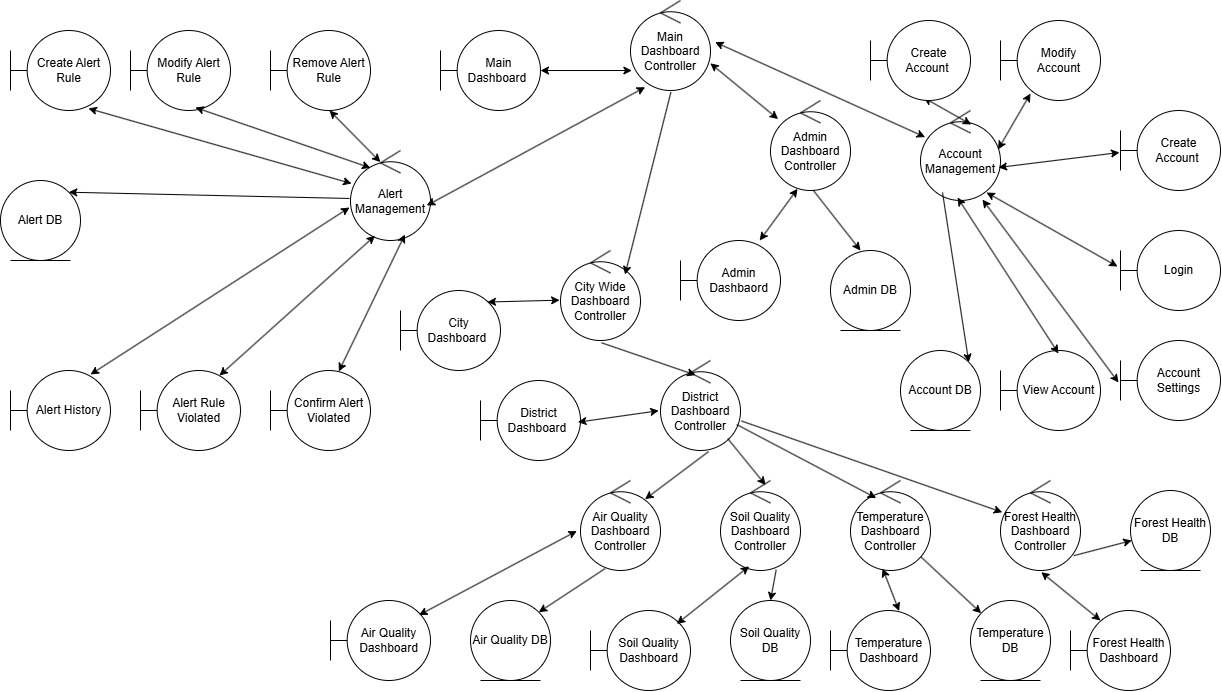
\includegraphics[width=1\textwidth]{./assets/analysis class.jpg}
    \caption{Analysis Class Diagram}
    \label{fig:analysis-class}
\end{figure}
% End Section

\newpage
\section{Architectural Design}
\label{sec:architectural_design}
% Begin Section
% This section should provide an overview of the overall architectural design of your application. Your overall architecture should show the division of the system into subsystems with high cohesion and low coupling.
This section provides an overview of the overall architectural design of SCEMAS.

\subsection{System Architecture}
\label{sub:system_architecture}
\begin{figure}[H]
    \centering
    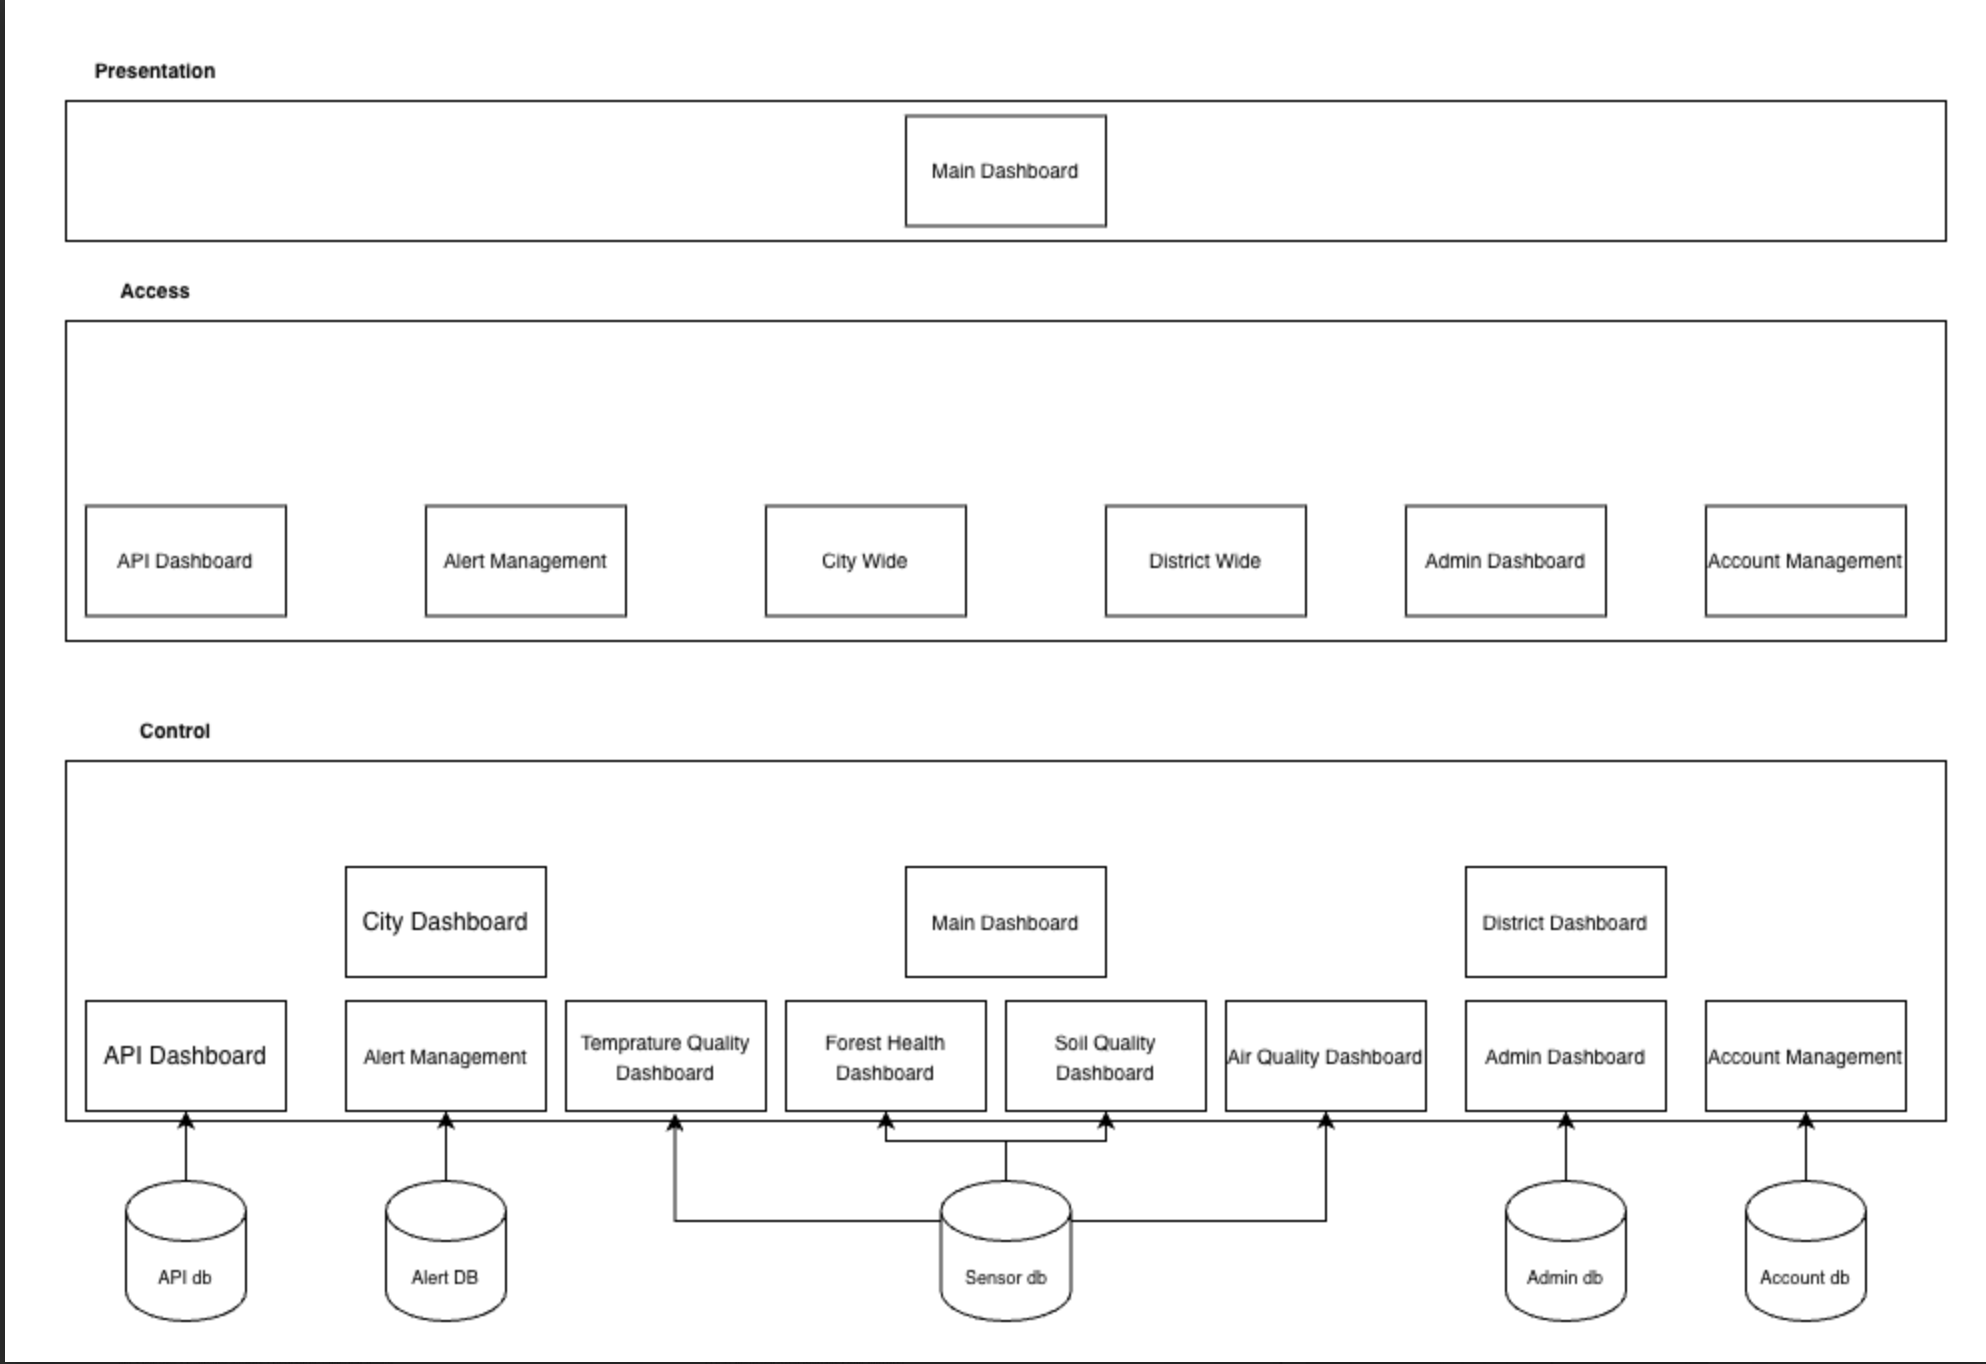
\includegraphics[width=\textwidth]{./assets/d2_arch_diagram.png}
    \caption{Structural Architecture Diagram for SCEMAS}
    \label{fig:architecture-diagram}
\end{figure}

% Begin SubSection
% \begin{itemize}
% 	\item Identify and explain the overall architecture of your system
% 	\item Be sure to clearly state the name of the architecture you used (this is the name of the architectural pattern, not the name of your system)
% 	\item Provide the reasoning and justification of the choice of architecture
% 	\item Provide a structural architecture diagram showing the relationship among the subsystems (if appropriate)
% 	\item List any design alternatives you considered, but eliminated (and explain why you eliminated them)
% \end{itemize}

\subsubsection{Choice of Architecture} 
SCEMAS utilizes an Interaction-Oriented Software Architecture, specifically the Presentation-Abstraction-Control (PAC) architecture style, in combination with the 
Data-Centered Repository architecture style. The PAC structure supports SCEMAS's interactive and interface-driven behaviour, while the Repository acts as the centralized 
data backbone that stores all environmental telemetry, alert information, administrative data, and account records. \\

\noindent The PAC architecture was selected, as it separates an interactive system into a hierarchy of cooperating agents, each with its own presentation logic, abstraction 
logic, and control component. This structure aligns well with SCEMAS, where multiple interactive components must operate independently while still coordinating at a higher level. PAC allows each component to maintain high cohesion, as each agent encapsulates its own interaction and domain logic. At the same time, it minimizes coupling between agents, as communication flows strictly through their controllers. This supports flexibility, ease of extension, and adherence to the Open-Closed Principle: new dashboards, alert interfaces, or user-facing views can be added as independent PAC agents without requiring modification of the existing structure. \\

\noindent The Repository architecture complements PAC by providing a passive, centralized data store with consistent and uniform access mechanisms. All environmental readings, alert rules, alert histories, and account-related data are contained within the repository. This allows PAC agents to retrieve and update data without needing to coordinate with each other; hence, this passive data store ensures low coupling between subsystems. The repository also supports data integrity, scalability, and concurrency, all of which are required for real-time environmental monitoring. The combination of PAC and the Repository thus establishes a system with strong modularity, high cohesion in each interactive agent, and low coupling across subsystem boundaries. \\

\noindent Within the main system controller, several high-level architectural groupings are defined as summarized in Table~\ref{tab:arch-overview}. These groupings reflect the interaction-oriented agents and the centralized repositories that support them.


\begin{table}[H]
\centering
\caption{Overview of Architectural Groupings in SCEMAS}
\label{tab:arch-overview}
\begin{tabular}{|p{4cm}|p{6.5cm}|p{4cm}|}
\hline
\textbf{Grouping} & \textbf{Purpose} & \textbf{Architectural Style} \\
\hline
Alert & Store alert rules, alert history, and violation events & Repository \\
\hline
Account & Maintain user accounts, authentication data, and role permissions & Repository \\
\hline
Admin & Maintain administrative configurations and internal system records & Repository \\
\hline
% Interactive Agents & Handle user interactions, visual displays, and control logic for system features & PAC \\
% \hline
Sensor Data & Store sensor readings, environmental metrics, and related data & Repository \\
\hline
\end{tabular}
\end{table}

\subsubsection{Considered Design Alternatives} 
\textbf{Model-View-Controller (MVC)} \\
The MVC architectural pattern was considered because the system uses web dashboards to display environmental data. MVC is best used to organize interactive applications where a single central model supports multiple views, and user interactions are the main concern of the system. It is especially well suited for UI-based systems that focus on maintaining consistency between the interface and data. The SCEMAS software contains multiple complex components (telemetry ingestion, alert management, rule evaluation, etc.), which each have their own logic and control flow, with data changing and different periods and frequencies. As these components must be coordinated at a system level, is is challenging to maintain the structure with a PAC architecture. MVC assumes a centralized structure between the model, view, and controller, which does not support the hierarchical structure that PAC offers. \\

\noindent \textbf{Blackboard} \\
The Blackboard architecture was considered since the system involves multiple subsystems that interact with a centralized data store. Blackboard is most appropriate for subsystems in which agents collaborate by contributing partial solutions to a problem stored in the blackboard. 
This architecture was eliminated since SCEMAS does not involve collaborative problem-solving among knowledge sources. Its subsystems do not compete, or contribute partial solutions. Instead, interactions with the data store are agent-driven, through read and writes. The data store therefore simply acts as passive storage. Since there is no need for agents to incrementally work on a shared solution state, the blackboard would simply introduce unnecessary coordination complexity. \\

\noindent \textbf{Batch Sequential Architecture} \\
The Batch Sequential Architecture is designed for systems that process data in discrete batches. Each processing stage must complete before the next stage starts, meaning that data flows linearly. SCEMAS, however, requires real-time (continuous) processing of environmental telemetry. Sensor data must be evaluated in real time to generate rule violations and environmental alerts without delay. Since the Batch Sequential architecture relies on periodic batch execution, it would introduce latency and prevent timely alert generation. Therefore, the Batch Sequential architecture was not selected. \\

\noindent \textbf{Additional Data Flow Architectures} \\
The Pipe-and-Filter and Process-Control architectural styles were not considered as design alternatives because they had not yet been introduced in the course lectures when the architectures were discussed.
% End SubSection

\subsection{Subsystems}
\label{sub:subsystems}
% Begin SubSection
The system has been divided into four primary subsystems: 
\begin{enumerate}
    \item Alert Management
    \item Account Management 
    \item Dashboard
    \item Public API
\end{enumerate}
\subsubsection{Alert Management Subsystem}
The Alert Management subsystem is responsible for evaluating the environmental data against the predefined rules and generating alerts when the system detects a threshold violation. This may include environmental events such as wildfire risks, extreme heat conditions, or potential for natural disasters, such as hurricanes. The subsystem manages the life cycle of these alerts, including when they are created, confirmed, and resolved. It is also responsible for maintaining a history of all logged alerts and their current status. This isolation of concerns helps to ensure high-cohesion of alert functionalities, and maintain loose coupling with storage and presentation components.\\

\noindent This subsystem is responsible for interacting with the Repository and Dashboard subsystem. It needs to communicate with the Repository to retrieve the environmental data required for alert evaluation. Its interactions with the Dashboard are essential to provide real-time updates on the status of a particular alert. When a threshold violation is detected, the subsystem generates a corresponding alert event, which is uploaded to the dashboard for City Operators to view. 
% End SubSection

\subsubsection{Account Management Subsystem}
The Account Management subsystem is responsible for authenticating and authorizing the different users of the system and ensuring that role-based access control (RBAC) is sustained. It allows users to register, log in, and manage their account details. It also defines the different user roles (city operators, public users) and ensures that only those who have permission to access a specific functionality are able to do so. Separating these details into its own subsystem is essential to help enhance the overall security while ensuring that authentication operates independently. \\

\noindent Like the Alert Management subsystem, it also needs to collaborate with the Repository. This is needed to securely store user information and profile details.
% End SubSection

\subsubsection{Dashboard Subsystem}
The dashboard subsystem is essential for providing an interface to display environmental data and alerts. It displays the real-time sensor readings, paleographical maps, sensor locations, and environmental metrics. This is fundamental for allowing city operators to monitor environmental conditions and make necessary responses. \\

\noindent The Dashboard subsystem interacts with the Alert Management subsystem to display current and historical alerts. It also communicates with the Repository to retrieve environmental data and metrics. The Dashboard subsystem follows the Presentation Abstraction Control (PAC) architecture pattern to separate user interface elements, interaction logic, and data models. 
% End SubSection

\subsubsection{Public API Subsystem}
The Public API subsystem provides controlled access to environmental data and alert information through its REST endpoints. Third-party developers and public users can request to retrieve environmental data and relevant alert information generated by the system. \\

\noindent This subsystem primarily communicates with the Alert Management and Repository subsystems. To satisfy client requests, it retrieves environmental and alert data from the Repositories. It also collects alert data generated by the Alert Management subsystem to ensure that alerts stay up to date when the public wants to view them. By separating how this data is accessed externally, with a separate subsystem, the architecture keeps internal system components loosely coupled with external users.
% End SubSection
% End Section

\newpage
\section{Class Responsibility Collaboration (CRC) Cards}
\label{sec:class_responsibility_collaboration_crc_cards}
% Begin Section
% This section should contain all of your CRC cards.

\begin{table}[H]
    \centering
    \caption{CRC Card for Main Dashboard Controller}
    \vspace{1mm}
    \begin{tabular}{|p{7.5cm}|p{7.5cm}|}
    \hline 
      \multicolumn{2}{|l|}{\textbf{Class Name: Main Dashboard Controller}} \\
    \hline
    \textbf{Responsibility:} & \textbf{Collaborators:} \\
    \hline
        Knows Main Dashboard \newline
        Knows Account Management \newline
        Knows Admin Dashboard Controller \newline
        Knows Alert Management \newline
        Knows API Controller \newline
        Knows API Controller \newline
        Facilitates communication regarding overall dashboard structure \newline
        &
        Main Dashboard \newline
        Account Management \newline
        Admin Dashboard Controller \newline
        Alert Management \newline
        PI Controller \\
    \hline
    \end{tabular}
\end{table}
\begin{table}[H]
    \centering
    \caption{CRC Card for Alert Management Controller}
    \vspace{1mm}
    \begin{tabular}{|p{7.5cm}|p{7.5cm}|}
    \hline 
      \multicolumn{2}{|l|}{\textbf{Class Name: Alert Management Controller}} \\
    \hline
    \textbf{Responsibility:} & \textbf{Collaborators:} \\
    \hline
        Knows Alert Database \newline
        Knows Create Alert Rule \newline
        Knows Modify Alert Rule \newline 
        Knows Remove Alert Rule \newline
        Knows Alert Rule Violated \newline
        Knows Confirm Alert Rule Violated \newline
        Knows Alert History \newline
        & 
        Alert Database \newline
        Create Alert Rule \newline
        Modify Alert Rule \newline 
        Remove Alert Rule \newline
        Alert Rule Violated \newline
        Confirm Alert Rule Violated \newline
        Alert History \\
    \hline
    \end{tabular}
\end{table}
\begin{table}[H]
    \centering
    \caption{CRC Card for Alert Database Entity}
    \vspace{1mm}
    \begin{tabular}{|p{7.5cm}|p{7.5cm}|}
    \hline 
     \multicolumn{2}{|l|}{\textbf{Class Name: Alert Database (Entity)}} \\
    \hline
    \textbf{Responsibility:} & \textbf{Collaborators:} \\
    \hline
        Knows Alert Management \newline
        Handles overall alert storage \newline
        & 
        Alert Management \\
    \hline
    \end{tabular}
\end{table}
\begin{table}[H]
    \centering
    \caption{CRC Card for Creating an Alert Rule}
    \vspace{1mm}
    \begin{tabular}{|p{7.5cm}|p{7.5cm}|}
    \hline 
      \multicolumn{2}{|l|}{\textbf{Class Name: Create Alert Rule (Boundary)}} \\
    \hline
    \textbf{Responsibility:} & \textbf{Collaborators:} \\
    \hline
        Handles interfacing for creating new alert rules \newline
        Collects and validates alert rule parameters \newline
        Sends the creation request to the Alert Management Controller \newline     
        & 
        Alert Management Controller \\
    \hline
    \end{tabular}
\end{table}
\begin{table}[H]
    \centering
    \caption{CRC Card for Modifying an Alert Rule}
    \vspace{1mm}
    \begin{tabular}{|p{7.5cm}|p{7.5cm}|}
    \hline 
      \multicolumn{2}{|l|}{\textbf{Class Name: Modify Alert Rule (Boundary)}} \\
    \hline
    \textbf{Responsibility:} & \textbf{Collaborators:} \\
    \hline
        Handles interfacing for updating alert rules \newline
        Displays current rule information \newline
        Validates rule modifications \newline
        Sends the modification request to the Alert Management Controller \newline
        & 
        Alert Management Controller \\
    \hline
    \end{tabular}
\end{table}
\begin{table}[H]
    \centering
    \caption{CRC Card for Removing an Alert Rule}
    \vspace{1mm}
    \begin{tabular}{|p{7.5cm}|p{7.5cm}|}
    \hline 
      \multicolumn{2}{|l|}{\textbf{Class Name: Remove Alert Rule (Boundary)}} \\
    \hline
    \textbf{Responsibility:} & \textbf{Collaborators:} \\
    \hline
        Handles interfacing for deleting an alert rule \newline
        Allows users to select an alert rule for removal \newline
        Sends deletion request to the Alert Management Controller \newline
        & 
        Alert Management Controller \\
    \hline
    \end{tabular}
\end{table}
\begin{table}[H]
    \centering
    \caption{CRC Card for Alert History}
    \vspace{1mm}
    \begin{tabular}{|p{7.5cm}|p{7.5cm}|}
    \hline 
      \multicolumn{2}{|l|}{\textbf{Class Name: Alert History (Boundary)}} \\
    \hline
    \textbf{Responsibility:} & \textbf{Collaborators:} \\
    \hline
        Knows Alert Management \newline
        Handles alert log storage \newline        
        & 
        Alert Management \\
    \hline
    \end{tabular}
\end{table}
\begin{table}[H]
    \centering
    \caption{CRC Card for Alert Rule Violation}
    \vspace{1mm}
    \begin{tabular}{|p{7.5cm}|p{7.5cm}|}
    \hline 
      \multicolumn{2}{|l|}{\textbf{Class Name: Alert Rule Violated (Boundary)}} \\
    \hline
    \textbf{Responsibility:} & \textbf{Collaborators:} \\
    \hline
        Notifies the system when environmental data violates an alert rule \newline
        Sends violation notifications to dashboards or user \newline
        Sends violation information to the Alert Management Controller \newline
        & 
        Alert Management Controller \\
    \hline
    \end{tabular}
\end{table}
\begin{table}[H]
    \centering
    \caption{CRC Card for Confirming an Alert Rule Violation}
    \vspace{1mm}
    \begin{tabular}{|p{7.5cm}|p{7.5cm}|}
    \hline 
      \multicolumn{2}{|l|}{\textbf{Class Name: Confirm Alert Rule Violated (Boundary)}} \\
    \hline
    \textbf{Responsibility:} & \textbf{Collaborators:} \\
    \hline
        Allow city operators to confirm a detected alert violation \newline
        Display the details of the alert event \newline
        Send confirmation status to the Alert Management Controller \newline
        & 
        Alert Management Controller \\
    \hline
    \end{tabular}
\end{table}
\begin{table}[H]
    \centering
    \caption{CRC Card for Main Dashboard}
    \vspace{1mm}
    \begin{tabular}{|p{7.5cm}|p{7.5cm}|}
    \hline 
      \multicolumn{2}{|l|}{\textbf{Class Name: Main Dashboard}} \\
    \hline
    \textbf{Responsibility:} & \textbf{Collaborators:} \\
    \hline
        Knows Main Dashboard Controller \newline
        Handles display of main dashboard \newline
        & 
        Main Dashboard Controller \\
    \hline
    \end{tabular}
\end{table}
\begin{table}[H]
    \centering
    \caption{CRC Card for API Controller}
    \vspace{1mm}
    \begin{tabular}{|p{7.5cm}|p{7.5cm}|}
    \hline 
      \multicolumn{2}{|l|}{\textbf{Class Name: API Controller}} \\
    \hline
    \textbf{Responsibility:} & \textbf{Collaborators:} \\
    \hline
        Knows API Documentation \newline
        Knows API Database \newline
        Knows Main Dashboard Controller \newline
        Facilitates communication and implementation of API calls \newline
        &
        API Documentation \newline
        API Database \newline
        Main Dashboard Controller \\
    \hline
    \end{tabular}
\end{table}
\begin{table}[H]
    \centering
    \caption{CRC Card for API Documentation}
    \vspace{1mm}
    \begin{tabular}{|p{7.5cm}|p{7.5cm}|}
    \hline 
      \multicolumn{2}{|l|}{\textbf{Class Name: API Documentation}} \\
    \hline
    \textbf{Responsibility:} & \textbf{Collaborators:} \\
    \hline
        Knows API Controller \newline
        Responsible for displaying API documentation for developers \newline
        &
        API Controller \\
    \hline
    \end{tabular}
\end{table}
\begin{table}[H]
    \centering
    \caption{CRC Card for API Database}
    \vspace{1mm}
    \begin{tabular}{|p{7.5cm}|p{7.5cm}|}
    \hline 
      \multicolumn{2}{|l|}{\textbf{Class Name: API Database}} \\
    \hline
    \textbf{Responsibility:} & \textbf{Collaborators:} \\
    \hline
        Knows API Controller \newline
        Knows Endpoints \newline
        Knows active and inactive routes \newline
        &
        API Controller \\          
    \hline
    \end{tabular}
\end{table}   
\begin{table}[H]
    \centering
    \caption{CRC Card for Admin Dashboard Controller}
    \vspace{1mm}
    \begin{tabular}{|p{7.5cm}|p{7.5cm}|}
    \hline 
      \multicolumn{2}{|l|}{\textbf{Class Name: Admin Dashboard Controller}} \\
    \hline
    \textbf{Responsibility:} & \textbf{Collaborators:} \\
    \hline
        Knows Main Dashboard Controller & Main Dashboard \\
        Knows Admin Dashboard & Admin Dashboard \\
        Knows Admin DB & Admin DB \\ 
    \hline
    \end{tabular}
\end{table}   
\begin{table}[H]
    \centering
    \caption{CRC Card for Admin Dashboard}
    \vspace{1mm}
    \begin{tabular}{|p{7.5cm}|p{7.5cm}|}
    \hline 
      \multicolumn{2}{|l|}{\textbf{Class Name: Admin Dashboard}} \\
    \hline
    \textbf{Responsibility:} & \textbf{Collaborators:} \\
    \hline
        Knows Admin Dashboard Controller & Admin Dashboard Controller \\
        Responsible for displaying administrator action interface & \\
    \hline
    \end{tabular}
\end{table}  
\begin{table}[H]
    \centering
    \caption{CRC Card for Admin Database}
    \vspace{1mm}
    \begin{tabular}{|p{7.5cm}|p{7.5cm}|}
    \hline 
      \multicolumn{2}{|l|}{\textbf{Class Name: Admin Database}} \\
    \hline
    \textbf{Responsibility:} & \textbf{Collaborators:} \\
    \hline
        Knows Admin Dashboard Controller & Admin Dashboard Controller \\
        Knows Admin privileges & \\
        Knows Admin action log history & \\
    \hline
    \end{tabular}
\end{table}
\begin{table}[H]
    \centering
    \caption{CRC Card for City Wide Dashboard Controller}
    \vspace{1mm}
    \begin{tabular}{|p{7.5cm}|p{7.5cm}|}
    \hline 
      \multicolumn{2}{|l|}{\textbf{Class Name: City Wide Dashboard Controller}} \\
    \hline
    \textbf{Responsibility:} & \textbf{Collaborators:} \\
    \hline
        Knows City Wide Dashboard & City Wide Dashboard\\
        Knows Main Dashboard Controller & Main Dashboard Controller\\
        Knows District Dashboard Controller & District Dashboard Controller \\
    \hline
    \end{tabular}
\end{table}
\begin{table}[H]
    \centering
    \caption{CRC Card for City Dashboard}
    \vspace{1mm}
    \begin{tabular}{|p{7.5cm}|p{7.5cm}|}
    \hline 
      \multicolumn{2}{|l|}{\textbf{Class Name: City Dashboard}} \\
    \hline
    \textbf{Responsibility:} & \textbf{Collaborators:} \\
    \hline
    Knows City Dashboard Controller \newline
    Handles display of city dashboard \newline
    & 
    City Dashboard Controller \\
    \hline
    \end{tabular}
\end{table}   
\begin{table}[H]
    \centering
    \caption{CRC Card for Account Management Controller}
    \vspace{1mm}
    \begin{tabular}{|p{7.5cm}|p{7.5cm}|}
    \hline 
    \multicolumn{2}{|l|}{\textbf{Class Name: Account Management Controller}} \\
    \hline
    \textbf{Responsibility:} & \textbf{Collaborators:} \\
    \hline
        Knows Create Account \newline
        Knows Modify Account \newline
        Knows Login \newline
        Knows Account Settings \newline
        Knows View Account \newline
        Knows Account Database \newline
        Knows Main Dashboard Controller \newline
        Coordinates validation, persistence, and retrieval for account features
        &
        Create Account \newline
        Modify Account \newline
        Login \newline
        Account Settings \newline
        View Account \newline
        Account Database \newline
        Main Dashboard Controller \\
    \hline
    \end{tabular}
\end{table}
\begin{table}[H]
    \centering
    \caption{CRC Card for Creating an Account}
    \vspace{1mm}
    \begin{tabular}{|p{7.5cm}|p{7.5cm}|}
    \hline 
    \multicolumn{2}{|l|}{\textbf{Class Name: Create Account (Boundary)}} \\
    \hline
    \textbf{Responsibility:} & \textbf{Collaborators:} \\
    \hline
        Handles interfacing for creating new accounts \newline
        Collects and validates registration parameters \newline
        Provides user feedback on password and policy compliance \newline
        Sends the creation request to the Account Management Controller
        &
        Account Management Controller \\
    \hline
    \end{tabular}
\end{table}
\begin{table}[H]
    \centering
    \caption{CRC Card for Modifying an Account}
    \vspace{1mm}
    \begin{tabular}{|p{7.5cm}|p{7.5cm}|}
    \hline 
    \multicolumn{2}{|l|}{\textbf{Class Name: Modify Account (Boundary)}} \\
    \hline
    \textbf{Responsibility:} & \textbf{Collaborators:} \\
    \hline
        Handles interfacing for updating account details \newline
        Displays current account information \newline
        Validates profile and credential modifications \newline
        Sends the modification request to the Account Management Controller
        &
        Account Management Controller \\
    \hline
    \end{tabular}
\end{table}
\begin{table}[H]
    \centering
    \caption{CRC Card for Login}
    \vspace{1mm}
    \begin{tabular}{|p{7.5cm}|p{7.5cm}|}
    \hline 
    \multicolumn{2}{|l|}{\textbf{Class Name: Login (Boundary)}} \\
    \hline
    \textbf{Responsibility:} & \textbf{Collaborators:} \\
    \hline
        Handles interfacing for user authentication \newline
        Collects and validates credentials \newline
        Manages error messaging for failed attempts \newline
        Sends the authentication request to the Account Management Controller
        &
        Account Management Controller \\
    \hline
    \end{tabular}
\end{table}
\begin{table}[H]
    \centering
    \caption{CRC Card for Account Settings}
    \vspace{1mm}
    \begin{tabular}{|p{7.5cm}|p{7.5cm}|}
    \hline 
    \multicolumn{2}{|l|}{\textbf{Class Name: Account Settings (Boundary)}} \\
    \hline
    \textbf{Responsibility:} & \textbf{Collaborators:} \\
    \hline
        Handles interfacing for configuring account preferences \newline
        Displays current settings \newline
        Validates and applies preference changes \newline
        Sends the update request to the Account Management Controller
        &
        Account Management Controller \\
    \hline
    \end{tabular}
\end{table}

\begin{table}[H]
    \centering
    \caption{CRC Card for Viewing an Account}
    \vspace{1mm}
    \begin{tabular}{|p{7.5cm}|p{7.5cm}|}
    \hline 
    \multicolumn{2}{|l|}{\textbf{Class Name: View Account (Boundary)}} \\
    \hline
    \textbf{Responsibility:} & \textbf{Collaborators:} \\
    \hline
        Handles interfacing for viewing account profile and status \newline
        Requests and renders account data \newline
        Sends data fetch requests to the Account Management Controller
        &
        Account Management Controller \\
    \hline
    \end{tabular}
\end{table}
\begin{table}[H]
    \centering
    \caption{CRC Card for Account Database Entity}
    \vspace{1mm}
    \begin{tabular}{|p{7.5cm}|p{7.5cm}|}
    \hline 
    \multicolumn{2}{|l|}{\textbf{Class Name: Account Database (Entity)}} \\
    \hline
    \textbf{Responsibility:} & \textbf{Collaborators:} \\
    \hline
        Knows Account Management Controller \newline
        Handles overall account storage \newline
        Persists account records, credentials, and settings \newline
        Supports retrieval, updates, and deletion of account data
        &
        Account Management Controller \\
    \hline
    \end{tabular}
\end{table}
\begin{table}[H]	
    \centering
    \caption{CRC Card for District Dashboard Controller}
    \vspace{1mm}
    \begin{tabular}{|p{7.5cm}|p{7.5cm}|}
    \hline 
    \multicolumn{2}{|l|}{\textbf{Class Name: District Dashboard Controller}} \\
    \hline
    \textbf{Responsibility:} & \textbf{Collaborators:} \\
    \hline
        Knows City Wide Dashboard Controller \newline
        Knows District Dashboard \newline
        Knows Air Quality Dashboard Controller \newline
        Knows Soil Quality Dashboard Controller \newline
        Knows Temperature Dashboard Controller \newline
        Knows Forest Health Dashboard Controller \newline
        Coordinates navigation within the district dashboard \newline
        Routes requests from the district dashboard to the correct environmental dashboard controller \newline
        Aggregates district-level environmental information for presentation
        &
        City Wide Dashboard Controller \newline
        District Dashboard \newline
        Air Quality Dashboard Controller \newline
        Soil Quality Dashboard Controller \newline
        Temperature Dashboard Controller \newline
        Forest Health Dashboard Controller \\
    \hline
    \end{tabular}
\end{table} 
\begin{table}[H]
    \centering
    \caption{CRC Card for District Dashboard}
    \vspace{1mm}
    \begin{tabular}{|p{7.5cm}|p{7.5cm}|}
    \hline 
    \multicolumn{2}{|l|}{\textbf{Class Name: District Dashboard}} \\
    \hline
    \textbf{Responsibility:} & \textbf{Collaborators:} \\
    \hline
        Knows District Dashboard Controller \newline
        Displays district-level environmental information \newline
        Handles user selection of district environmental categories \newline
        Sends user navigation requests to the District Dashboard Controller
        &
        District Dashboard Controller \\
    \hline
    \end{tabular}
\end{table}
\begin{table}[H]
    \centering
    \caption{CRC Card for Air Quality Dashboard Controller}
    \vspace{1mm}
    \begin{tabular}{|p{7.5cm}|p{7.5cm}|}
    \hline 
    \multicolumn{2}{|l|}{\textbf{Class Name: Air Quality Dashboard Controller}} \\
    \hline
    \textbf{Responsibility:} & \textbf{Collaborators:} \\
    \hline
        Knows District Dashboard Controller \newline
        Knows Air Quality Dashboard \newline
        Knows Air Quality Database \newline
        Retrieves air quality data for the selected district \newline
        Processes air quality data for presentation \newline
        Updates the Air Quality Dashboard with district-specific results
        &
        District Dashboard Controller \newline
        Air Quality Dashboard \newline
        Air Quality Database \\
    \hline
    \end{tabular}
\end{table}
\begin{table}[H]
    \centering
    \caption{CRC Card for Air Quality Dashboard}
    \vspace{1mm}
    \begin{tabular}{|p{7.5cm}|p{7.5cm}|}
    \hline 
    \multicolumn{2}{|l|}{\textbf{Class Name: Air Quality Dashboard}} \\
    \hline
    \textbf{Responsibility:} & \textbf{Collaborators:} \\
    \hline
        Knows Air Quality Dashboard Controller \newline
        Displays district air quality information \newline
        Handles user requests to view air quality metrics \newline
        Presents processed air quality data to the user
        &
        Air Quality Dashboard Controller \\
    \hline
    \end{tabular}
\end{table}
\begin{table}[H]
    \centering
    \caption{CRC Card for Air Quality Database}
    \vspace{1mm}
    \begin{tabular}{|p{7.5cm}|p{7.5cm}|}
    \hline 
    \multicolumn{2}{|l|}{\textbf{Class Name: Air Quality Database}} \\
    \hline
    \textbf{Responsibility:} & \textbf{Collaborators:} \\
    \hline
        Knows Air Quality Dashboard Controller \newline
        Stores district air quality data \newline
        Provides requested air quality records \newline
        Maintains air quality measurement history
        &
        Air Quality Dashboard Controller \\
    \hline
    \end{tabular}
\end{table}
\begin{table}[H]
    \centering
    \caption{CRC Card for Soil Quality Dashboard Controller}
    \vspace{1mm}
    \begin{tabular}{|p{7.5cm}|p{7.5cm}|}
    \hline 
    \multicolumn{2}{|l|}{\textbf{Class Name: Soil Quality Dashboard Controller}} \\
    \hline
    \textbf{Responsibility:} & \textbf{Collaborators:} \\
    \hline
        Knows District Dashboard Controller \newline
        Knows Soil Quality Dashboard \newline
        Knows Soil Quality Database \newline
        Retrieves soil quality data for the selected district \newline
        Processes soil quality data for presentation \newline
        Updates the Soil Quality Dashboard with district-specific results
        &
        District Dashboard Controller \newline
        Soil Quality Dashboard \newline
        Soil Quality Database \\
    \hline
    \end{tabular}
\end{table}
\begin{table}[H]
    \centering
    \caption{CRC Card for Soil Quality Dashboard}
    \vspace{1mm}
    \begin{tabular}{|p{7.5cm}|p{7.5cm}|}
    \hline 
    \multicolumn{2}{|l|}{\textbf{Class Name: Soil Quality Dashboard}} \\
    \hline
    \textbf{Responsibility:} & \textbf{Collaborators:} \\
    \hline
        Knows Soil Quality Dashboard Controller \newline
        Displays district soil quality information \newline
        Handles user requests to view soil quality metrics \newline
        Presents processed soil quality data to the user
        &
        Soil Quality Dashboard Controller \\
    \hline
    \end{tabular}
\end{table}
\begin{table}[H]
    \centering
    \caption{CRC Card for Soil Quality Database}
    \vspace{1mm}
    \begin{tabular}{|p{7.5cm}|p{7.5cm}|}
    \hline 
    \multicolumn{2}{|l|}{\textbf{Class Name: Soil Quality Database}} \\
    \hline
    \textbf{Responsibility:} & \textbf{Collaborators:} \\
    \hline
        Knows Soil Quality Dashboard Controller \newline
        Stores district soil quality data \newline
        Provides requested soil quality records \newline
        Maintains soil quality measurement history
        &
        Soil Quality Dashboard Controller \\
    \hline
    \end{tabular}
\end{table}
\begin{table}[H]
    \centering
    \caption{CRC Card for Temperature Dashboard Controller}
    \vspace{1mm}
    \begin{tabular}{|p{7.5cm}|p{7.5cm}|}
    \hline 
    \multicolumn{2}{|l|}{\textbf{Class Name: Temperature Dashboard Controller}} \\
    \hline
    \textbf{Responsibility:} & \textbf{Collaborators:} \\
    \hline
        Knows District Dashboard Controller \newline
        Knows Temperature Dashboard \newline
        Knows Temperature Database \newline
        Retrieves temperature data for the selected district \newline
        Processes temperature data for presentation \newline
        Updates the Temperature Dashboard with district-specific results
        &
        District Dashboard Controller \newline
        Temperature Dashboard \newline
        Temperature Database \\
    \hline
    \end{tabular}
\end{table}
\begin{table}[H]
    \centering
    \caption{CRC Card for Temperature Dashboard}
    \vspace{1mm}
    \begin{tabular}{|p{7.5cm}|p{7.5cm}|}
    \hline 
    \multicolumn{2}{|l|}{\textbf{Class Name: Temperature Dashboard (Boundary)}} \\
    \hline
    \textbf{Responsibility:} & \textbf{Collaborators:} \\
    \hline
        Knows Temperature Dashboard Controller \newline
        Displays district temperature information \newline
        Handles user requests to view temperature metrics \newline
        Presents processed temperature data to the user
        &
        Temperature Dashboard Controller \\
    \hline
    \end{tabular}
\end{table}
\begin{table}[H]
    \centering
    \caption{CRC Card for Temperature Database}
    \vspace{1mm}
    \begin{tabular}{|p{7.5cm}|p{7.5cm}|}
    \hline 
    \multicolumn{2}{|l|}{\textbf{Class Name: Temperature Database}} \\
    \hline
    \textbf{Responsibility:} & \textbf{Collaborators:} \\
    \hline
        Knows Temperature Dashboard Controller \newline
        Stores district temperature data \newline
        Provides requested temperature records \newline
        Maintains temperature measurement history
        &
        Temperature Dashboard Controller \\
    \hline
    \end{tabular}
\end{table}
\begin{table}[H]
    \centering
    \caption{CRC Card for Forest Health Dashboard Controller}
    \vspace{1mm}
    \begin{tabular}{|p{7.5cm}|p{7.5cm}|}
    \hline 
    \multicolumn{2}{|l|}{\textbf{Class Name: Forest Health Dashboard Controller}} \\
    \hline
    \textbf{Responsibility:} & \textbf{Collaborators:} \\
    \hline
        Knows District Dashboard Controller \newline
        Knows Forest Health Dashboard \newline
        Knows Forest Health Database \newline
        Retrieves forest health data for the selected district \newline
        Processes forest health data for presentation \newline
        Updates the Forest Health Dashboard with district-specific results
        &
        District Dashboard Controller \newline
        Forest Health Dashboard \newline
        Forest Health Database \\
    \hline
    \end{tabular}
\end{table}
\begin{table}[H]
    \centering
    \caption{CRC Card for Forest Health Dashboard}
    \vspace{1mm}
    \begin{tabular}{|p{7.5cm}|p{7.5cm}|}
    \hline 
    \multicolumn{2}{|l|}{\textbf{Class Name: Forest Health Dashboard}} \\
    \hline
    \textbf{Responsibility:} & \textbf{Collaborators:} \\
    \hline
        Knows Forest Health Dashboard Controller \newline
        Displays district forest health information \newline
        Handles user requests to view forest health metrics \newline
        Presents processed forest health data to the user
        &
        Forest Health Dashboard Controller \\
    \hline
    \end{tabular}
    \end{table}
\begin{table}[H]
    \centering
    \caption{CRC Card for Forest Health Database}
    \vspace{1mm}
    \begin{tabular}{|p{7.5cm}|p{7.5cm}|}
    \hline 
    \multicolumn{2}{|l|}{\textbf{Class Name: Forest Health Database}} \\
    \hline
    \textbf{Responsibility:} & \textbf{Collaborators:} \\
    \hline
        Knows Forest Health Dashboard Controller \newline
        Stores district forest health data \newline
        Provides requested forest health records \newline
        Maintains forest health measurement history
        &
        Forest Health Dashboard Controller \\
    \hline
    \end{tabular}
\end{table}
% End Section

\newpage
\appendix
\section{Division of Labour}
\label{sec:division_of_labour}
% Begin Section

\noindent \textbf{Benjamin Bloomfield} 
\begin{itemize}
    \item Took part in discussion of chosen architectures.
    \item Took part in discussion of chosen subsystems. 
    \item 3.1: Justification of considered architectures that were not chosen.
    \item 3.2.1 Subsystem descriptions.
    \item 4. CRC Cards:
    \begin{itemize}
        \item Formatted all tables
        \item Alert Management Controller
        \item Create Alert Rule 
        \item Modify Alert Rule 
        \item Remove Alert Rule
        \item Alert Rule Violated
        \item Confirm Alert Rule Violated
    \end{itemize}

    \vspace{0.5cm}
    \centering
    
\includegraphics[width=10cm]{./signatures/ben_bloomfield_signature.jpg}
    \\\vspace{0.2cm}
    Date: March 8th, 2026
    \vspace{0.5cm}
\end{itemize}


\noindent \textbf{Vikram Chandar}
\begin{itemize}
    \item Section 2: Analysis Class Diagram
    \item Created cards for each class for Section 4
    \item 4. CRC Cards:
    \begin{itemize}
        \item Main Dashboard
        \item Main Dashboard Controller
        \item Admin Dashboard Controller
        \item Admin Dashboard
        \item Admin DB
        \item API Controller
        \item API DB
        \item API Documentation
    \end{itemize}
\end{itemize}

\vspace{0.5cm}
    \centering
    
\includegraphics[width=10cm]{./signatures/IMG_4568.jpg}
    \\\vspace{0.2cm}
    Date: March 8th, 2026 
\vspace{0.5cm}

\noindent \textbf{Trisha Panchal}
\begin{itemize}
    \item 3.1:
	\begin{itemize}
		\item Identification and justification of the choice of overall architecture.
		\item Considered design alternatives.
		\item Structural architecture diagram.
	\end{itemize}
	\item 4. CRC Cards:
	\begin{itemize}
		\item Account Management Controller
		\item Create Account
		\item Modify Account
		\item Login
		\item Account Settings
		\item View Account
		\item Account Database
	\end{itemize}

    \vspace{0.5cm}
    \centering
    
\includegraphics[width=10cm]{./signatures/trisha_d1_sign.jpg}
    \\\vspace{0.2cm}
    Date: March 8th, 2026
    \vspace{0.5cm}
\end{itemize}

\noindent \textbf{Yug Vashisth}
\begin{itemize}
    \item Section 3.1: Structural architecture diagram
    \item Section 4. CRC Cards:
    \begin{itemize}
        \item District Dashboard Controller
        \item District Dashboard
        \item Air Quality Dashboard Controller
        \item Air Quality Dashboard
        \item Air Quality DB
        \item Soil Quality Dashboard Controller
        \item Soil Quality Dashboard
        \item Soil Quality DB
        \item Temperature Dashboard Controller
        \item Temperature Dashboard
        \item Temperature DB
        \item Forest Health Dashboard Controller
        \item Forest Health Dashboard
        \item Forest Health DB
    \end{itemize}
\vspace{0.5cm}
    \centering
    
\includegraphics[width=10cm]{./signatures/yug_sig.jpg}
    \\\vspace{0.2cm}
    Date: March 8th, 2026
\vspace{0.5cm}	
\end{itemize}

\noindent \textbf{Hamza Nadeem}
\begin{itemize}
    \item Section 1
    \item Created cards for each class for Section 4
    \item 4. CRC Cards:
    \begin{itemize}
        \item Alert Database
        \item Alert History
        \item Main Dashboard
        \item City Wide Dashboard Controller
        \item City Wide Dashboard
    \end{itemize}
\end{itemize}

\vspace{0.5cm}
    \centering
    
\includegraphics[width=5cm]{signatures/hamza_nadeem_signature.jpeg}
    \\\vspace{0.2cm}
    Date: March 8th, 2026
\vspace{0.5cm}
% End Section


\end{document}
%------------------------------------------------------------------------------